
\documentclass[13pt,compress]{beamer}
% deactivate beamer navigation
%\setbeamertemplate{navigation symbols}{}
%\usepackage{geometry}
%\geometry{papersize={180mm, 135mm}, top=-1.5mm} % 210mm, 297mm

\usepackage[nospeakermargin]{../../style/lmu-lecture}

\setbeamertemplate{frametitle}{\expandafter\uppercase\expandafter\insertframetitle}
%\useoutertheme{metropolis}
% remove section slides
\AtBeginSection[]
{
  \begin{frame}<beamer>
    \frametitle{Supervised Learning I}
    \tableofcontents[currentsection]
  \end{frame}
}
% includepdf slides, pagecommad will set counter for framenumber
\usepackage{pdfpages}
\includepdfset{trim=0mm 0mm 0mm 0mm, pagecommand={\global\setcounter{framenumber}{\value{page}}}}
% trim=0mm 6mm 0mm 0mm, offset=0 15,
% add footer:
\usepackage{framed, color}
\usepackage{xcolor}
%\iffalse
\setbeamertemplate{footline}[text line]{%
    \noindent\hspace*{\dimexpr-\oddsidemargin-1in\relax}%
     \colorbox{white}{
     \makebox[\dimexpr\paperwidth-2\fboxsep\relax]{
     \color{black}
     \begin{minipage}[c][4.5ex][c]{0.5\linewidth}
       \secname
     \end{minipage}
     \hfill\begin{minipage}[c][4.5ex][c]{0.5\linewidth}
       \flushright
       \insertframenumber{}~/~\inserttotalframenumber~~
     \end{minipage}
     }}%
  \hspace*{-\paperwidth}
}
%\fi

\title{Supervised Learning I}
\author{Essential Data Science Training}
%\institute{Essential Data Science Training}
\date{}



\begin{document}
\setbeamercolor{background canvas}{bg=}

% General remark: hyperlinks in included pdfs are not clickable anymore in the combined pdf

\frame{\titlepage}

\section{Introduction}
\includepdf[pages={2-3}, trim=0mm 0mm 45mm 0mm]{../../material/lecture_i2ml/slides-pdf/slides-basics-nutshell.pdf}
\includepdf[pages={3-4}, trim=0mm 0mm 45mm 0mm]{../../material/lecture_i2ml/slides-pdf/slides-basics-data.pdf}
\includepdf[pages={4}, trim=0mm 0mm 45mm 0mm]{../../material/lecture_i2ml/slides-pdf/slides-basics-nutshell.pdf}
\includepdf[pages={8-9}, trim=0mm 0mm 45mm 0mm]{../../material/lecture_i2ml/slides-pdf/slides-basics-models-parameters.pdf}
\includepdf[pages={2, 4-last}, trim=0mm 0mm 45mm 0mm]{../../material/lecture_i2ml/slides-pdf/slides-basics-learner.pdf}
\includepdf[pages={2}, trim=0mm 0mm 45mm 0mm]{../../material/lecture_i2ml/slides-pdf/slides-basics-riskminimization.pdf}
\includepdf[pages={7-8}, trim=0mm 0mm 45mm 0mm]{../../material/lecture_i2ml/slides-pdf/slides-basics-nutshell.pdf}
\section{Linear and Logistic Regression}
\includepdf[pages={2-5, 8}, trim=0mm 0mm 45mm 0mm]{../../material/lecture_i2ml/slides-pdf/slides-regression-nutshell.pdf}
\includepdf[pages={8-last}, trim=0mm 0mm 45mm 0mm]{../../material/lecture_i2ml/slides-pdf/slides-basics-riskminimization.pdf}
\includepdf[pages={2-4}, trim=0mm 0mm 45mm 0mm]{../../material/lecture_i2ml/slides-pdf/slides-classification-nutshell.pdf}
\includepdf[pages={2}, trim=0mm 0mm 45mm 0mm]{../../material/lecture_i2ml/slides-pdf/slides-classification-logistic.pdf}
\includepdf[pages={5}, trim=0mm 0mm 45mm 0mm]{../../material/lecture_i2ml/slides-pdf/slides-classification-nutshell.pdf}
\section{The KNN Learner}
\includepdf[pages={2-6}, trim=0mm 0mm 45mm 0mm]{../../material/lecture_i2ml/slides-pdf/slides-knn.pdf}
\section{Performance Estimation}
\includepdf[pages={2-3, 5}, trim=0mm 0mm 45mm 0mm]{../../material/lecture_i2ml/slides-pdf/slides-evaluation-generr.pdf}
\includepdf[pages={2,5-6}, trim=0mm 0mm 45mm 0mm]{../../material/lecture_i2ml/slides-pdf/slides-evaluation-train.pdf}
\includepdf[pages={2-5}, trim=0mm 0mm 45mm 0mm]{../../material/lecture_i2ml/slides-pdf/slides-evaluation-test.pdf}
\includepdf[pages={4}, trim=0mm 0mm 45mm 0mm]{../../material/lecture_i2ml/slides-pdf/slides-evaluation-overfitting-underfitting.pdf}
\section{Performance Measures}
\includepdf[pages={2-3, 5}, trim=0mm 0mm 45mm 0mm]{../../material/lecture_i2ml/slides-pdf/slides-evaluation-measures-regression.pdf}
\includepdf[pages={3}, trim=0mm 0mm 45mm 0mm]{../../material/lecture_i2ml/slides-pdf/slides-evaluation-measures-classification.pdf}
\includepdf[pages={7, 2-3, 10-11}, trim=0mm 0mm 45mm 0mm]{../../material/lecture_i2ml/slides-pdf/slides-evaluation-rocbasics.pdf}
\includepdf[pages={8}, trim=0mm 0mm 45mm 0mm]{../../material/lecture_i2ml/slides-pdf/slides-evaluation-measures-classification.pdf}
\includepdf[pages={12-13}, trim=0mm 0mm 45mm 0mm]{../../material/lecture_i2ml/slides-pdf/slides-evaluation-rocbasics.pdf}
\section{Introduction to mlr3}
\includepdf[pages={7-8, 10-18, 24, 26, 30-31, 33-36, 39-40, 42, 44-53, 55-59, 62-65, 67-71, last}]{../../material/mlr-doc/CURRENT_mlr3_course/01_mlr3/mlr3-intro.pdf}
\section{Exercise: Train, predict, evaluate}
\begin{frame}{Exercise: Train, predict, evaluate}
File: \textit{day1\_train\_predict\_evaluate.html}
\end{frame}
\section{Resampling}
\includepdf[pages={7}, trim=0mm 0mm 45mm 0mm]{../../material/lecture_i2ml/slides-pdf/slides-evaluation-generr.pdf}
\includepdf[pages={2, 7, 4, 6, 8}, trim=0mm 0mm 45mm 0mm]{../../material/lecture_i2ml/slides-pdf/slides-evaluation-resampling-1.pdf}
\includepdf[pages={last}, trim=0mm 0mm 45mm 0mm]{../../material/lecture_i2ml/slides-pdf/slides-evaluation-resampling-2.pdf}
\section{Resampling with mlr3}
\includepdf[pages={3, 5, 8-9, 11, 13, 18-23, 27-31}]{../../material/mlr-doc/CURRENT_mlr3_course/01_mlr3/mlr3-resampling.pdf}
\section{Exercise: Resampling with mlr3}
\begin{frame}{Exercise: Resampling with mlr3}
File: \textit{day1\_resampling.html}
\end{frame}
\section{Benchmarking with mlr3}
\includepdf[pages={33-36, 40-41, 43, 45-46, last}]{../../material/mlr-doc/CURRENT_mlr3_course/01_mlr3/mlr3-resampling.pdf}
\section{Exercise: Benchmarking with mlr3}
\begin{frame}{Exercise: Benchmarking with mlr3}
File: \textit{day1\_benchmarking.html}
\end{frame}



\end{document}
